\chapter{Introduction: Smartphone Market and the Need for Cross-Platform Support}
\label{chapter:introduction}

\section{Smartphone Landscape}
\label{section:smartphone-landscape}

\begin{table}
  \begin{tabular}{ l | l }
    \textbf{Mobile OS Type} & \textbf{Skill Set Required} \\
    \hline
    Apple iOS & C, Objective C \\
    Google Android & Java (Harmony flavored, Dalvik VM) \\
    RIM BlackBerry & Java (J2ME flavored) \\
    Symbian & C, C++, Python, HTML/CSS/JS \\
    Windows Mobile & .NET \\
    Windows 7 Phone & .NET \\
    HP Palm webOS & HTML/CSS/JS \\
    MeeGo & C, C++, HTML/CSS/JS \\
    Samsung bada & C++
  \end{tabular}
  \label{table:native-skills}
  \caption{Required skill sets for different mobile platforms. \cite{charland2011mobile}}
\end{table}

\section{HTML5}
\label{section:html5}

\subsection{History}
\subsection{Markup}
\subsection{CSS3}
\subsection{JavaScript APIs}
\subsection{Related APIs}

\section{Modern Mobile Web Application Architecture}
\label{section:modern-mobile-web}

\begin{figure}[ht]
  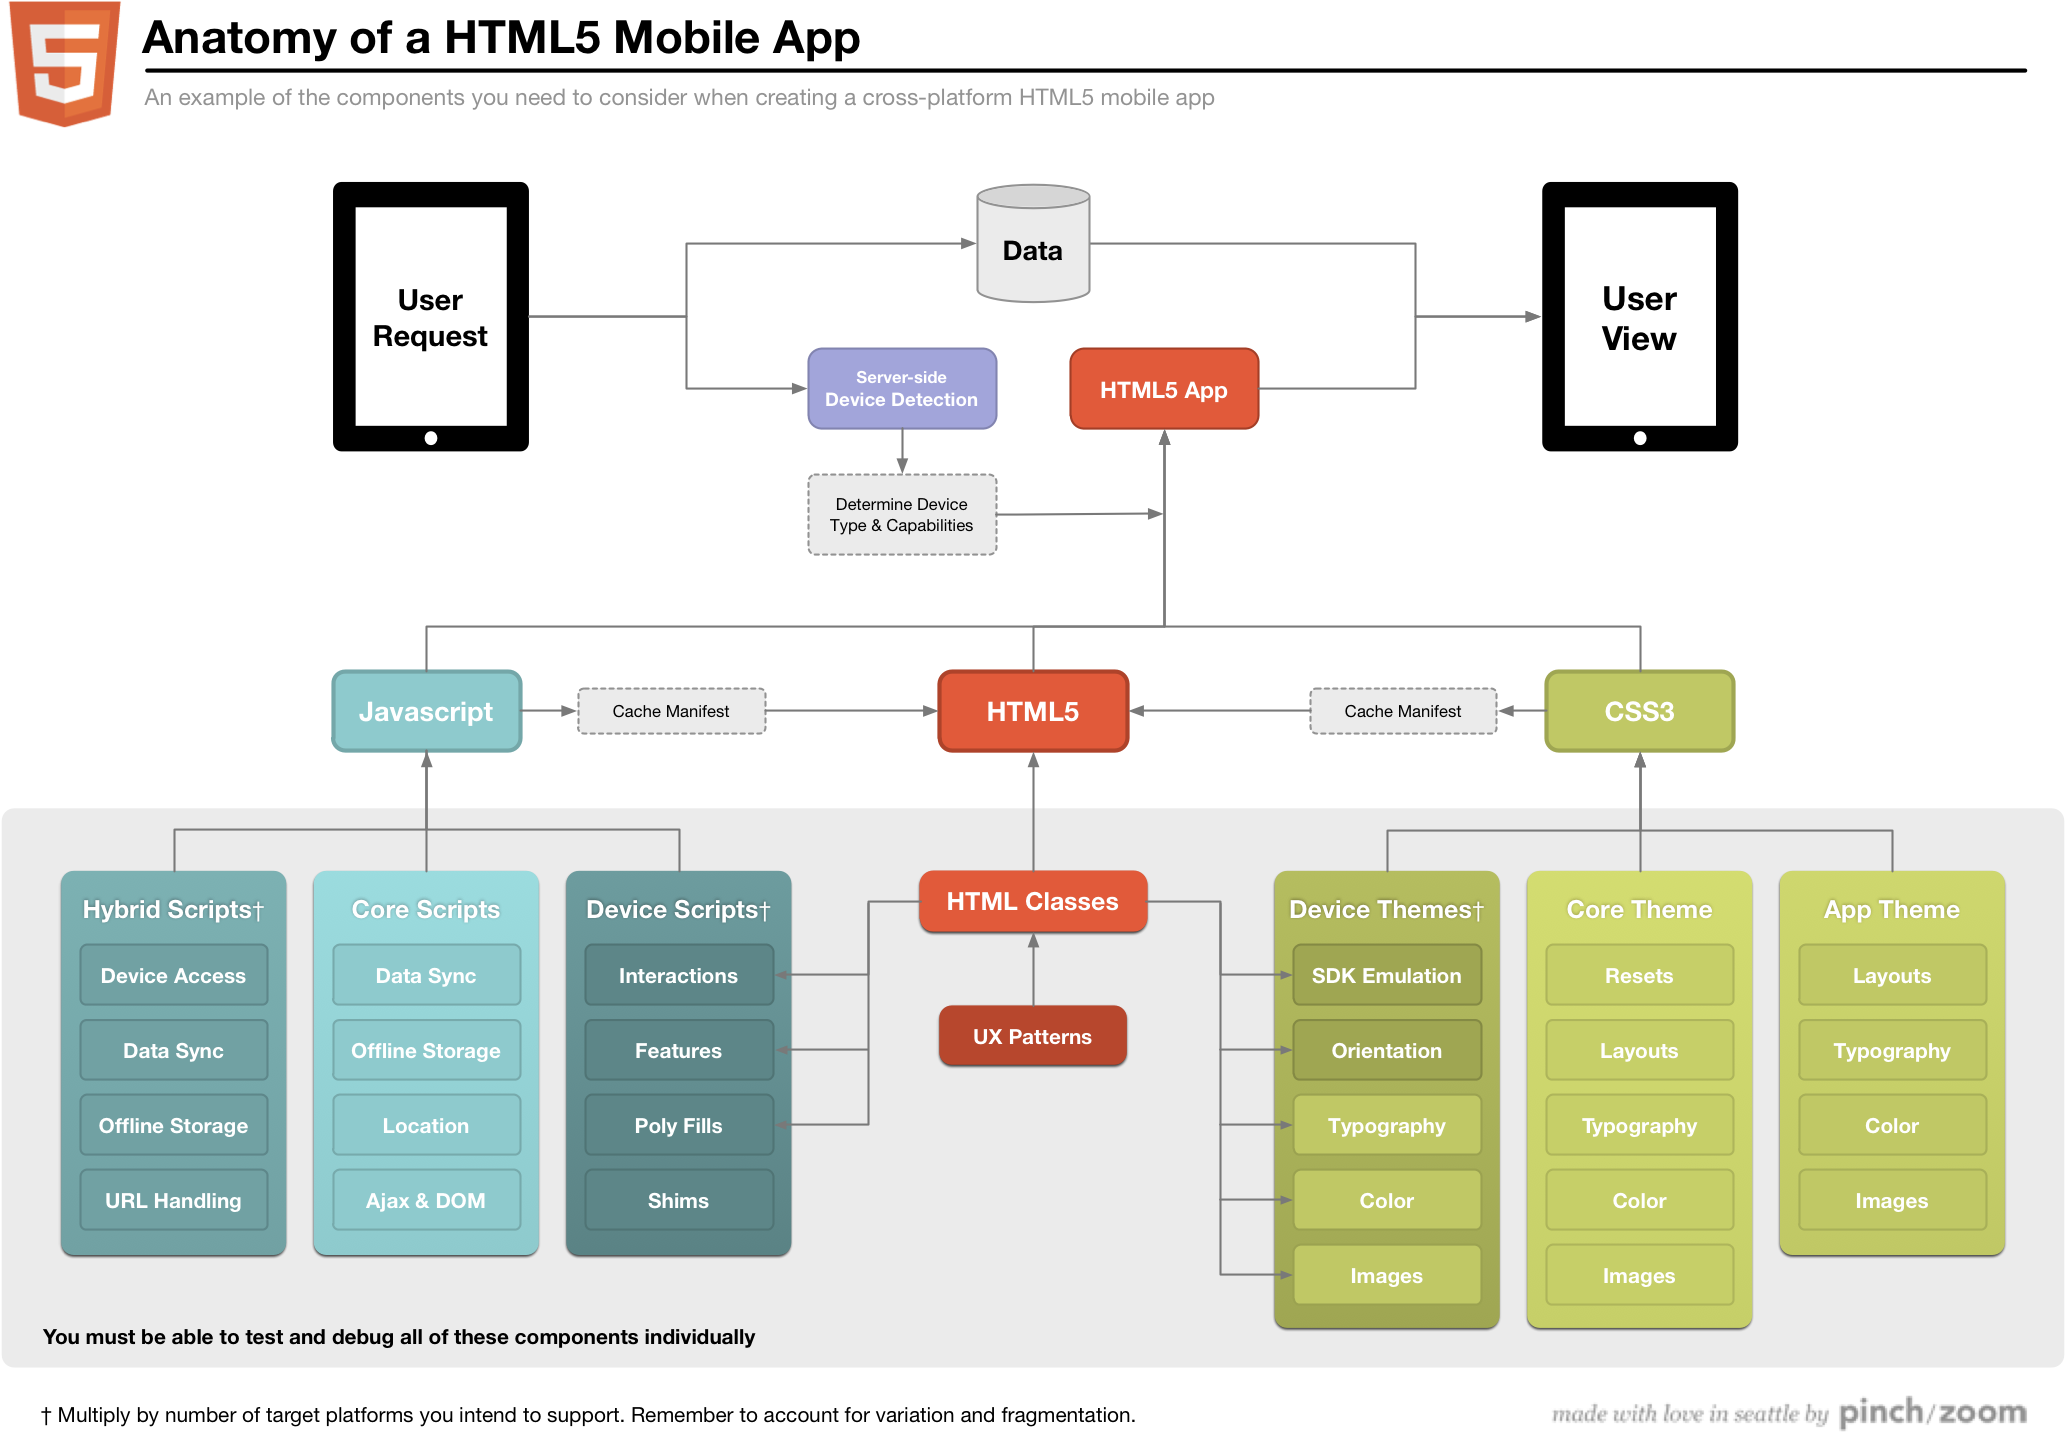
\includegraphics[width=\textwidth]{images/anatomy-of-a-html5-mobile-app.png}
  \caption{HTML5 Mobile Application Anatomy \citationneeded}
  \label{figure:anatomy-of-a-html5-mobile-app.png}
\end{figure}

\subsection{Single-Page applications}
\subsubsection{JavaScript MVC Libraries}

\subsection{Responsive Design}
\subsection{Progressive Enhancement}

\subsection{UI Libraries}
\subsubsection{jQuery Mobile}
\subsubsection{jQTouch}
\subsubsection{Sencha Touch}

\subsection{Hybrid Applications}
\subsection{Wrapping Web Applications Application Stores}

\section{Performance Guidelines}
\label{section:performance-guidelines}

\begin{itemize}
\item Make Fewer HTTP Requests
\item Use a Content Delivery Network
\item Add an Expires Header
\item Gzip Components
\item Put Stylesheets at the Top
\item Put Scripts at the Bottom
\item Avoid CSS Expressions
\item Make Javascript and CSS External
\item Reduce DNS Lookups
\item Minify JavaScript
\item Avoid Redirects
\item Remove Duplicate Scripts
\item Configure ETags
\item Make Ajax Cacheable
\item Splitting the Initial Payload
\item Loading Scripts Without Blocking
\item Coupling Asynchronous Scripts
\item Positioning Inline Scripts
\item Writing Efficient JavaScript
\item Scaling with Comet
\item Going Beyond Gzipping
\item Optimizing Images
\item Sharding Dominant Domains
\item Flushing the Document Early
\item Using Iframes Sparingly
\item Simplifying CSS Selectors
\end{itemize}
